\documentclass[12pt]{article}
\usepackage{amsmath}
\usepackage{url}
\usepackage{graphicx}
\graphicspath{{./img/}}
\usepackage{wrapfig}
\renewcommand{\arraystretch}{2.5}
\usepackage[numbers]{natbib}
\usepackage[czech]{babel}
\usepackage[T1]{fontenc}
\usepackage[utf8]{inputenc}
\title{FI-HMI: Temperovaná ladění}
\date{\today}
\author{Adam Havel}
\begin{document}

\maketitle

\pagebreak

\section{Absolutní a relativní sluch}

Každý alespoň trochu schopný muzikant by měl disponovat dobrým relativním sluchem, tedy schopností poznat frekvenční rozdíl mezi dvěma znějícími tóny a jen na základě poslechu rozhodnout, jaký hudební interval je odděluje. Takových intervalů je alespoň v naší klasické hudební nauce dvanáct, což je přirozeně stejné množství, jaké nám nabízí repertoár hudebních tónů neboli chromatická řada. A právě umění rozpoznat krom intervalu i samotné absolutní výšky, to znamená přiřadit je k jednomu z těchto dvanácti tónů — jako třeba C nebo G$\flat$ — se nazývá absolutním sluchem.

Většina lidí má představu, že je tato schopnost vrozená a spojuje si ji s jakýmsi přirozeným hudebním nadáním — ostatně jako příklad člověka, který byl tímto sluchem obdařen, se často udává třeba Wolfgang Amadeus Mozart. Jak ovšem zjistíme, s tímto \uv{Svatým grálem} muzikantů to není tak úplně jednoduché.

Dnes už tušíme, že se absolutní sluch formuje především v raném dětství a hlavní faktor představuje opakované vystavení hudebním tónům spolu s dalším podnětem, třeba vizuálním, který ke konkrétním zvukům přiřadí dané označení. Dětský mozek je pak schopen toto spojení zachovat a slyší-li pak jedinec, u kterého se tato vlastnost projeví, správnou frekvenci, na mysl mu okamžitě vytane i název tónu.

Problém ovšem nastane v momentě, kdy si uvědomíme, že frekvence jednotlivých tónů jsou jen předmětem úzu a momentální dohody a jejich hodnoty se tedy v průběhu času významně mění. Dnes se jako reference pro lazení nástrojů většinou používá takzvané koncertní A o hodnotě 440 Hz, nicméně to samé A bylo na počátku předchozího století skoro o deset hertzů menší. Podíváme-li se až do osmnáctého století, zjistíme dokonce, že se tato frekvence významně lišila nejen v čase, ale například i v rámci různých měst, a to i o desítky hertzů \cite{wiki_pitch}!

Ve světle těchto zjištění se absolutní sluch jeví jako svého druhu Danajský dar. V momentě, kdy orchestr ladí jinak, než je dnes zvyklé — třeba z důvodu větší autentičnosti u současných barokních souborů — slyší člověk s absolutním sluchem rozdíl a nepříjemně jej pociťuje. Nicméně, ani běžní posluchači nejsou ušetřeni následků změn hudebního úzu, protože se mění nejen tóny, ale i samotné vzdálenosti mezi nimi. Tyto intervaly určují matematicky odvozené systémy nazvané ladění, kterých v historii vzniklo velké množství: v hudební tradici naší západní kultury například dominuje takzvané rovnoměrně temperované ladění. Tak to ovšem nebylo vždy.

\pagebreak

\section{Harmonická řada}

Hudba, jak ji známe, by nemohla existovat nebýt jedné vlastnosti lidského mozku, a to sice té, že dva tóny vnímá jako v podstatě stejné, pokud jsou od sebe vzdáleny o interval oktávy. To jinými slovy znamená, že jsou jejich frekvence členy stejné geometrické posloupnosti o kvocientu 2 — jako A jsou tedy shodně označeny například tóny o frekvenci 440 a 220 Hz. Tuto vlastnost mimochodem sdílíme s mnoha dalšími savci \cite{octave_circularity}.

Ladění pak není nic jiného, než způsob, jak takto daný frekvenční rozsah rozdělit na jednotlivé tóny. Zde je důležité poznamenat, že ačkoliv v naší kultuře jsme zvyklí (už od Pythagora!) používat tónu dvanáct, jejich množství — ač podstatné — není pevně dané.

\begin{wrapfigure}{l}{0.4 \textwidth}\centering
	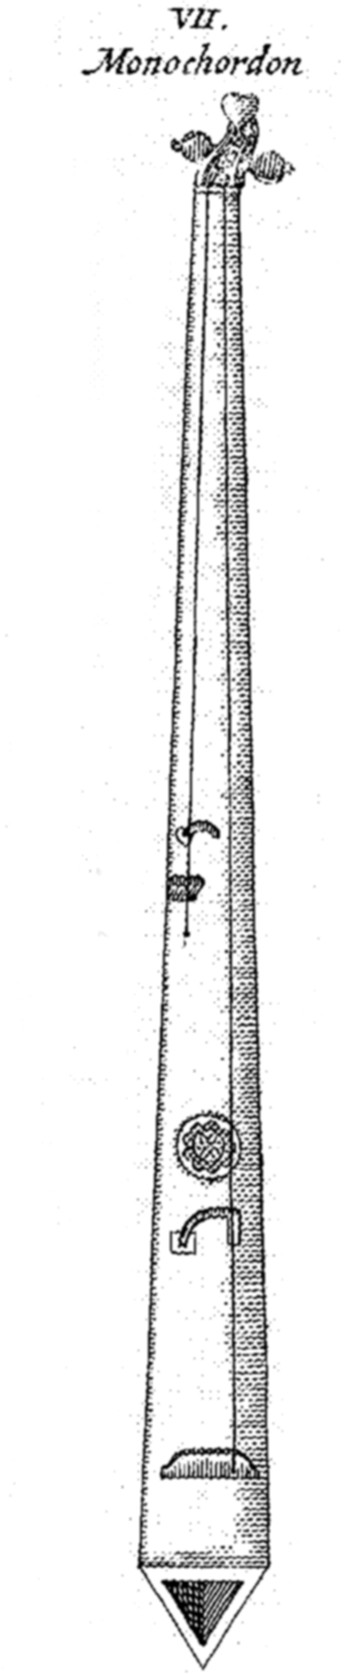
\includegraphics[width = 0.1 \textwidth]{monochord.jpg}
	\caption{Monochord}
	\label{fig:monochord}
\end{wrapfigure}

Právě Pythagorovi se pak přisuzuje jedno z nejstarších známých ladění, které se hojně používalo až do 16. století \cite{smolka}. Rozložení tónů v tomto systému bylo založeno na pozorování takzvaného \emph{monochordu}, což byl jednoduchý hudební — nebo spíše vědecký — nástroj o jedné (či více) strunách, určený k demonstraci vlastností tónů. S jeho pomocí tedy mohli zkoumat třeba výše zmíněnéný interval oktávy, a to tak, že strunu zkrátili na polovinu, čímž se frekvence tónu zdvojnásobila.

Řekové si tehdy všimli, že struna upevněná na obou koncích vibruje s frekvencí o vlnové délce rovné dvojnásobku délky struny — této frekvenci se říká \emph{fundemantální}. Ovšem mnohem důležitější bylo zjištění, že struna zároveň vibruje i s dalšími frekvencemi. První z nich má vlnovou délku rovnou délce struny, její frekvence je tedy dvákrat tak velká, což znamená, že jde o interval oktávy. Vibruje-li tedy struna se základní frekvencí 100 Hz, vibruje zároveň i s frekvencí dvojnásobnou, tedy 200 Hz. Jako další pozorujeme vibraci o 300 Hz, která je s předchozí oktavou v poměru 3:2 a jedná se o interval čisté kvinty. Jak můžeme vidět na obrázku ~\ref{fig:harmonics}, následující frekvence je zase oktáva, tentokrát o 400 Hz, a až po ní se objevuje nový tón, s frekvencí 500 Hz. Ten je s předchozí oktávou v poměru 5:4, jde tedy o velkou tercii. Poté následuje další kvinta a tak dále.

\begin{figure}[p]\centering
	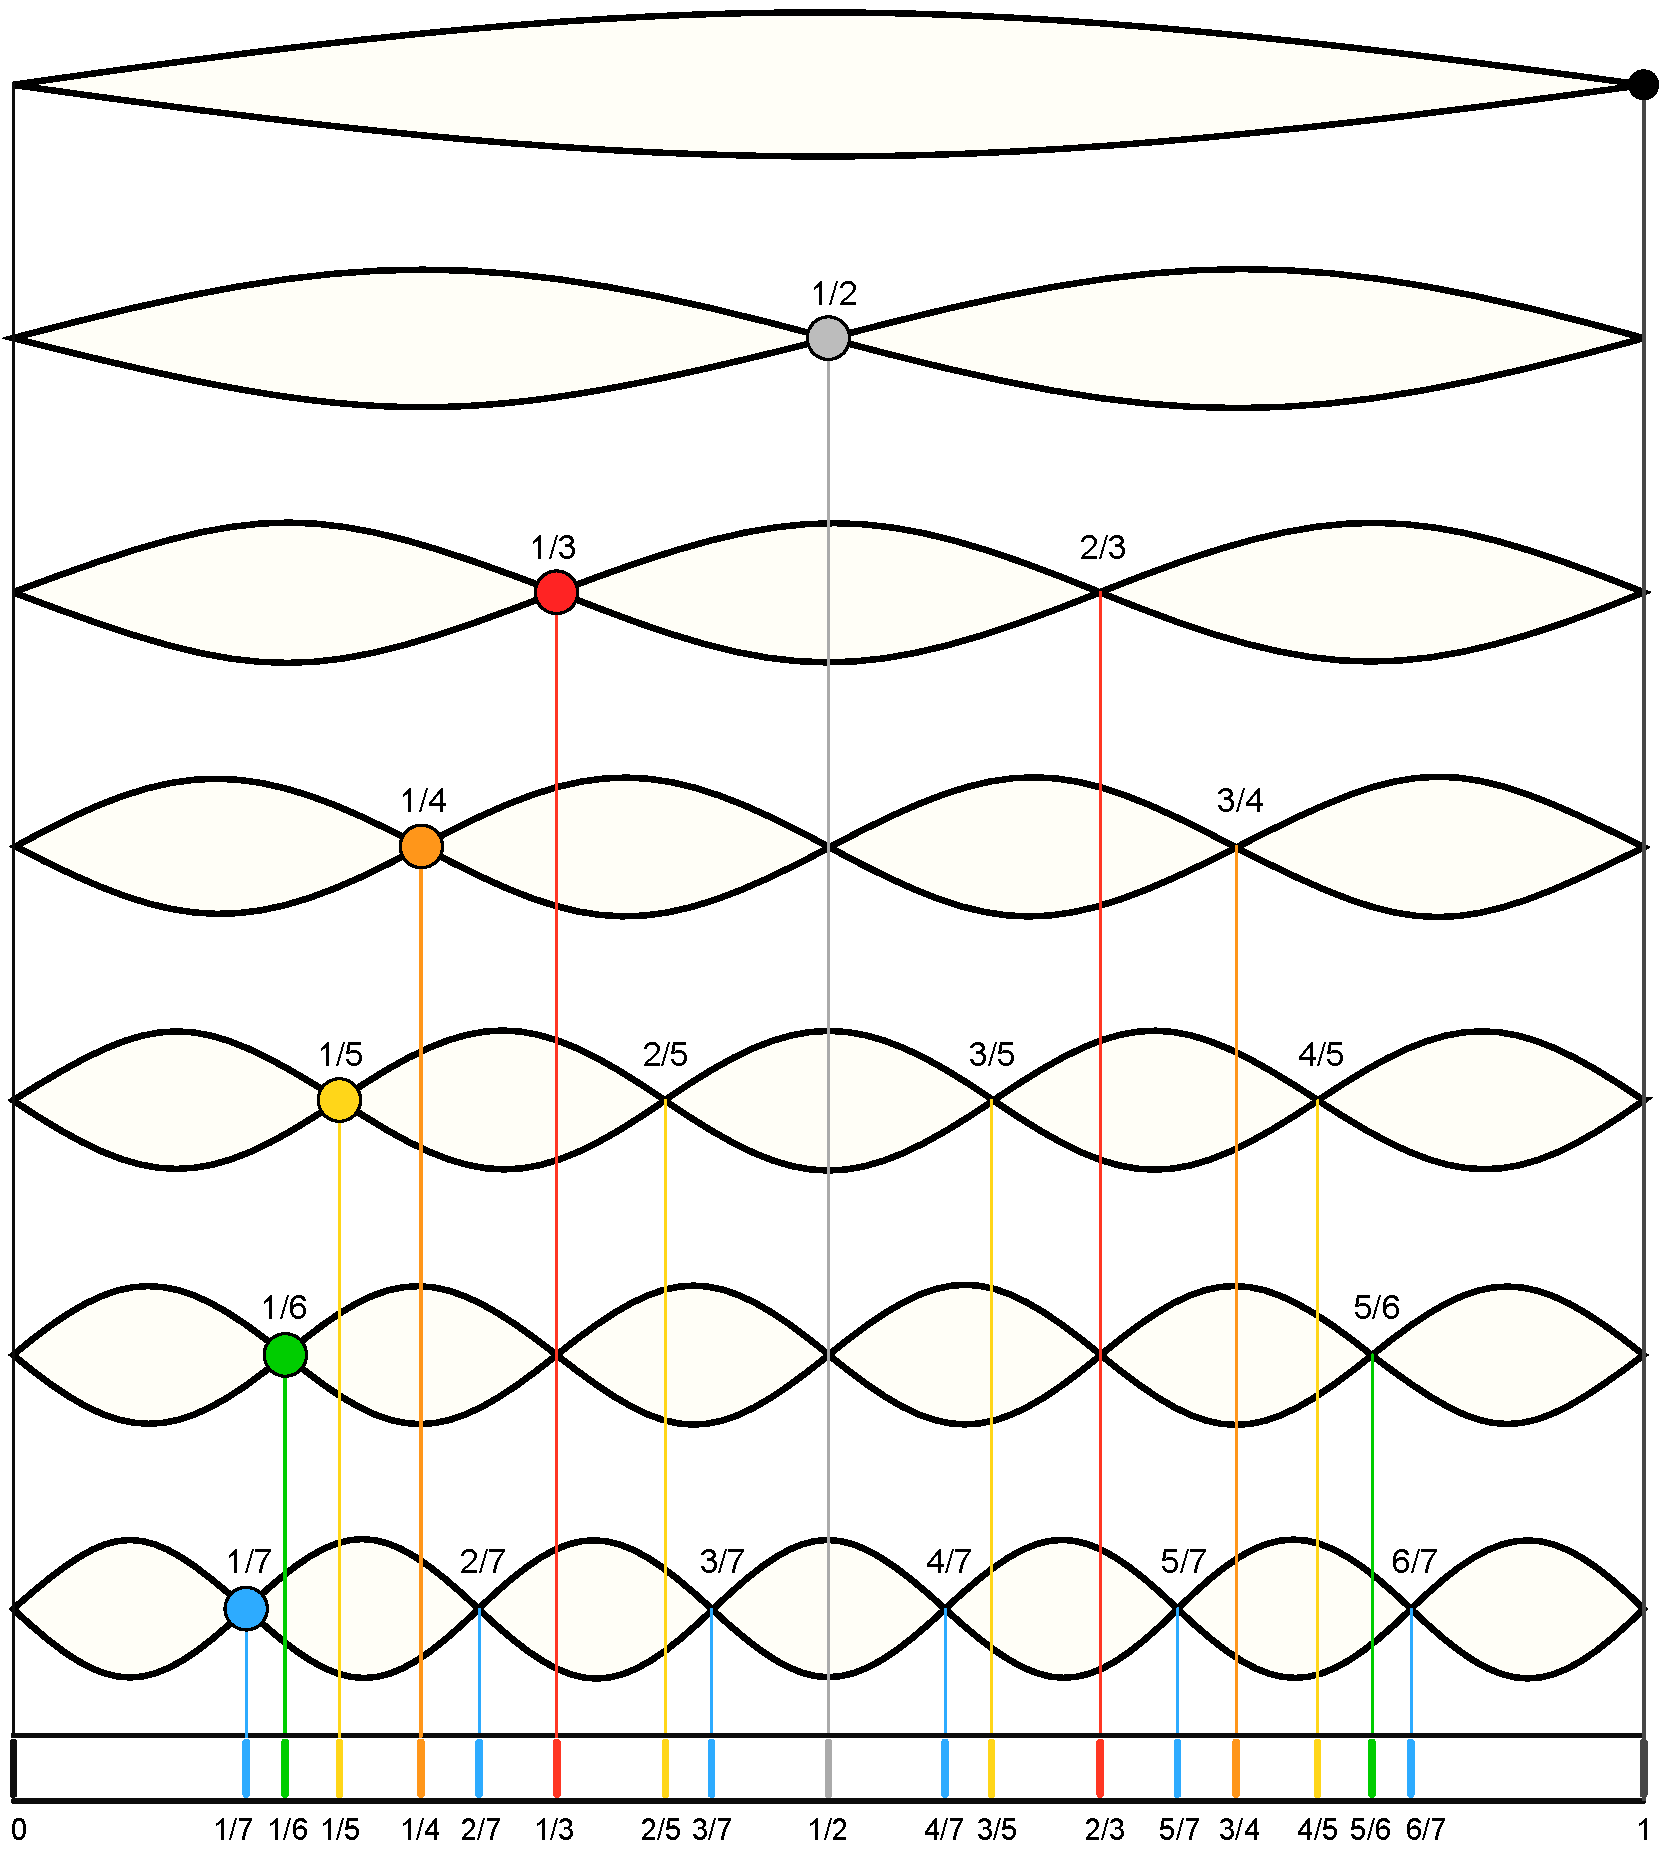
\includegraphics[width = .9 \textwidth]{harmonics.pdf}
	\caption{Harmonická řada (zdroj: Wikimedia)}
	\label{fig:harmonics}
\end{figure}

Tyto tóny se označují jako \emph{alikvótní} a jejich funkce je naprosto zásadní, protože jejich množství a intenzita v poměru k fundamentální frekvenci vytvářejí takzvanou barvu tónu. A právě díky barvě jsme jen podle sluchu schopni poznat hudební nástroj jeden od druhého. Některé, třeba flétna, disponují jen alikvótními tóny oktávy, jiné zase jen těmi lichými a podobně.

Než budeme pokračovat dále, je třeba si uvědomit několik poznatků. Zaprvé, alikvótní tóny jsou zjevně členy aritmetické posloupnosti o diferenci rovné fundamentální frekvenci. Zadruhé, vyšší oktávy a kvinty jsou nedílnou a podstatnou součastí většiny vibrujících těles. A zatřetí, jak postupujeme v harmonické řadě, objevují se stále menší intervaly a zlomky vyjadřující poměr k oktávám jsou čím dál složitější. Čistá kvinta s poměrem 3:2 je pak tedy hned po oktávě nejjednodušší interval. To je důležite i proto, že náš mozek vnímá intervaly, které se dají vyjádřit pomocí poměru malých čísel, jako stabilní. Naproti tomu ty intervaly, které mají ve zlomku velká čísla, považujeme za nepříjemné či nestabilní a nazýváme je disonantní.

Není proto náhodou, že nejstarší pentatonické stupnice (stupnice o pěti tónech) jsou založeny právě na intervalech přirozeně se vyskytujících v přírodě v podobě alikvótních tónů. Krom oktávy a kvinty jsou to velká tercie, čistá kvarta a malá septima. O tercii jsme se již zmínili, zaměříme se proto na poslední dva. Kvarta se ve skutečnosti v harmonické řadě objevuje až jako dvacátý alikvótní tón, ale dá se jednoduše matematicky odvodit ze svého vztahu ke kvintě. Jde totiž o její inverzi, což znamená, že složíme-li dohromady interval kvinty a kvarty, dostaneme oktávu. Víme-li, že kvinta je v poměru 3:2 a oktáva 2:1, můžeme si lehce odvodit, že kvarta představuje zlomek 4:3.

S přirozenou malou septimou je to složitější. Ta se v harmonické řadě objevuje jako šestý člen o poměru 7:4, což je pomerně odlišné číslo, než k jakému matematicky dospěli Řekové nebo jaké dnes používáme my v temperovaném ladění. Proto by se na dnešním klavíru tento interval zahrát nedal, neboť by ležel někde mezi velkou sextou a malou septimou. Jeho velikost se lišila i v rámci různých kultur, například v čínské tradici se používal interval srovnatelný s naší dnešní malou septimou, zatímco v té africké to naopak byla spíše velká sexta \cite{bernstein}. Ostatně v jazzu a blues, které z africké hudební tradice vycházejí, se u nástrojů, které to umožňují (tedy ne u klavíru), často používají takzvané \emph{blue} tóny, což není nic jiného, než \uv{ohnutí} použitého ladění k podobě blížší alikvótním tónům z přirozené harmonické řady.

\pagebreak

\section{Čistá ladění}

S předchozími znalostmi se konečně můžeme vrátit k Pythagorovi a jeho ladění, jehož základy stojí právě na intervalech oktávy a kvinty. Princip je takový, že všechny tóny vytvoříme jen skladáním těchto dvou intervalů. To znamená, že si vybereme tón, třeba D, a jeho frekvenci vynásobíme v poměru 3:2, čímž získáme interval kvinty a tón A. Od A postupujeme stejně, tedy násobíme 3:2. Tím se ovšem dostaneme mimo rozsah oktávy a proto frekvenci vydělíme dvěma. Výsledkem je tón E a interval velké sekundy s poměrem 9:8.
Stejným způsobem můžeme postupovat i směrem \uv{dolů} od základního D, akorát místo 3:2 násobíme v poměru 2:3, což značí snížení o interval kvinty. Abychom se vrátili do správné oktávy, musíme pak ještě výsledek vynásobit dvěma. Další výpočty pro ostatní tóny a jejich hodnoty jsou k vidění v tabulce ~\ref{tbl:pythagorean}. 

Již na první pohled zde vidíme zásadní problém — velká část intervalů je vyjádřena jako poměr relativně vysokých čísel a jak už jsme popsali výše, takové intervaly se našemu sluchu jeví jako velmi disonantní. Právě proto se v hudební tradici středověku, například v gregoriánských chorálech, objevují v podstatě jen intervaly oktávy, kvarty a kvinty \cite{smolka}. Tento problém částečně řeší jiné ladění, nazvané Didymické, které je \uv{čistší} než Pythagorejské, jelikož pro tvorbu tónu využívá i intervalů velké tercie a sexty, s poměry stanovenými na 5:4 a 5:3. To nicméně trpí zase jinými nedostatky.

Na druhý pohled zjistíme, že tónů je v tabulce třináct, na dvanáct, jak bychom očekávali. Na vině je fakt, že snížená kvinta a zvětšená kvarta je ve skutečnosti (alespoň v našem temperovaném ladění) jeden a ten samý interval, nazvaný \emph{tritón}, a tóny G$\sharp$ a A$\flat$ jsou takzvaně \emph{enharmonické}, neboli stejné. Podíváme-li se ovšem na jejich poměry v tabulce, zjistíme, že se liší — jedná se tedy o různé tóny.

\begin{table}[p]\centering
	\begin{tabular}{c c c c}
		\textbf{Tón} & \textbf{Interval} & \textbf{Výpočet} & \textbf{Poměr} \\ \hline
		A$\flat$ & snížená kvinta & $\left(\dfrac{2}{3}\right)^6 \times 2^4$ & $\dfrac{1024}{729}$ \\
		E$\flat$ & malá sekunda & $\left(\dfrac{2}{3}\right)^5 \times 2^3$ & $\dfrac{256}{243}$ \\
		B$\flat$ & malá sexta & $\left(\dfrac{2}{3}\right)^4 \times 2^3$ & $\dfrac{128}{81}$ \\
		F & malá tercie & $\left(\dfrac{2}{3}\right)^3 \times 2^2$ & $\dfrac{32}{27}$ \\
		C & malá septima & $\left(\dfrac{2}{3}\right)^2 \times 2^2$ & $\dfrac{16}{9}$ \\
		G & čistá kvarta & $\dfrac{2}{3} \times 2$ & $\dfrac{4}{3}$ \\
		D & čistá prima & $\dfrac{1}{1}$ & $\dfrac{1}{1}$ \\
		A & čistá kvinta & $\dfrac{3}{2}$ & $\dfrac{3}{2}$ \\
		E & velká sekunda & $\left(\dfrac{3}{2}\right)^2 \times \dfrac{1}{2}$ & $\dfrac{9}{8}$ \\
		B & velká sexta & $\left(\dfrac{3}{2}\right)^3 \times \dfrac{1}{2}$ & $\dfrac{27}{16}$ \\
		F$\sharp$ & velká tercie & $\left(\dfrac{3}{2}\right)^4 \times \left(\dfrac{1}{2}\right)^2$ & $\dfrac{81}{64}$ \\
		C$\sharp$ & velká septima & $\left(\dfrac{3}{2}\right)^5 \times \left(\dfrac{1}{2}\right)^2$ & $\dfrac{243}{128}$ \\
		G$\sharp$ & zvětšená kvarta & $\left(\dfrac{3}{2}\right)^6 \times \left(\dfrac{1}{2}\right)^3$ & $\dfrac{729}{512}$ \\
	\end{tabular}
	\caption{Pythagorejské ladění}
	\label{tbl:pythagorean}
\end{table}

Rozdílu mezi těmito dvěma tóny se říká \emph{Pythagorejské koma}. Jde o velmi malý interval, který si můžeme vyjádřit jako poměr dvanácti čistých kvint ku sedmi oktávám:

\begin{equation}
\dfrac{\left(3 : 2\right)^{12}}{\left(2 : 1\right)^7} = \dfrac{3^{12}}{2^{12 + 7}} = \dfrac{531441}{524288} \approx 1,01364
\end{equation}

Jeho velikost je tedy přibližně rovna čtvrt půltónu. Ke stejnému poměru bychom došli, pokud bychom dělili interval šesti velkých sekund, neboli $(9 : 8)^6$, oktávou, tedy dvěma. Ačkoliv by taková posloupnost sekund měla vést k čisté oktávě, výsledkem je zase interval o něco málo větší. Tímto způsobem ostatně ono koma objevil a spočítal již Euklides \cite{barker}.

Zde je ovšem třeba si znovu připomenout, že není vůbec nutné, aby oktáva měla přesně dvanáct tónů. Stejně tak dobře jich může mít pět. Nebo tisíc. Pro potřeby Pythagorejského tonálního systému je však toto číslo vhodné z toho důvodu, že není příliš velké — což usnadňuje konstrukci hudebních nástrojů a neklade tak velké nároky na muzikanty — a zároveň s uspokojivou přesností uzavíra takzvaný \emph{kvintový kruh}, až na zmíněné Pythagorejské koma.

Nicméně, už v roce zhruba 50 př. n. l. zjistil čínský matematik Ching Fang, že pokud se nezastavíme u dvanácté kvinty, ale pokračujeme až k její 53. iteraci, dostaneme systém, který kvintový kruh uzavírá s mnohem větší přesností. Výsledné koma, tentokrát nazvané po Nicholasu Mercatorovi, je pak zhruba rovné číslu 1,00209, což už je pro lidský sluch za hranicí rozlišitelnosti.

Pokud ovšem zůstaneme u klasické dvanáctitónové chromatické řady, s existencí onoho nezanedbatelného koma se musíme nějak vypořádat. V případě, kdy jako v tabulce ~\ref{tbl:pythagorean} vybereme za zákládní tón D, je klasický postup takový, že A$\flat$ nebereme v potaz a použijeme ostatních dvanáct tónů, které vznikly pomocí jedenácti čistých kvintových kroků. Zbývající dvanáctá kvinta mezi G$\sharp$ a E$\flat$ je o Pythagorejské koma větší a tedy nepoužitelná — takovému intervalu se říká \uv{vlčí}. Výsledkem je, že v takto postaveném ladění lze oba tyto tóny používat jen za cenu velkých disonancí. Samozřejmě, pokud bychom změnili tón, od kterého ostatní odvozujeme, vlčí interval by se posunul a nepoužitelné by byly zase jiné dva tóny.

Tato zjištění mají dvojí důsledek. Zaprvé kladou omezení na možnosti hudebního nástroje — při použití Pythagorejského ladění jsou vždy některé tóniny rozladěné a pokud je chceme použít, musíme nástroj přeladit. Tím se ovšem stávají nepoužitelné zase tóniny jiné a tak dále. Druhým následkem je fakt, že v rámci skladby nelze bez omezení modulovat, tedy přejít do jiné tóniny. A právě modulace je v soudobé hudbě zcela základní výrazový prostředek.

I přes tyto nedostatky však čístá ladění v určité formě přežívají i dnes — krom experimentálních použití je lze s úspěchem aplikovat na hudební nástroj nám nejbližší, a to sice lidské hlasivky. Ty totiž není třeba přelaďovat, záleží jen na umu a zkušenostech pěvce, což elegantně řeší hlavní neduh těchto ladění. Většina \emph{a capella} souborů proto přirozeně (a ne vždy záměrně) inklinuje k intervalům založených na jednoduchých zlomcích a z toho plynoucí velké konsonanci.
\pagebreak

\section{Temperovaná ladění}

\pagebreak

Baroko a cembalo (modulace, Bach, dur-mollové harmonie, konsonantní tercie a kvintakordy)

Temperovaná ladění (rozdílnost tónin)

Rovnoměrně temperované ladění (důvod, důsledky, matika)

Současnost


\bibliography{sources}{}
\bibliographystyle{plainnat}

\end{document}